% my main entry on the LaTeX report for my master thesis

\documentclass[a4paper]{report}
\usepackage[acronym,toc]{glossaries}
\usepackage{url}
\usepackage{graphicx}
\usepackage{float}
\usepackage{amssymb}

\makeglossaries

%my glossary (for the TM LHC tune)

\newglossaryentry{bunch}{
   name=bunch,
   description={
      particules trapped inside an \gls{RF} bucket circulating in the 
      machine},
   plural=bunches}
\newglossaryentry{bucket}{
   name={bucket},
   description={
      at every \gls{RF} period in the \gls{rffreq} there is a 
      bucket, in each of these bucket a particles bunch can potentially be 
      stored in the ring},
   plural={buckets}}
\newglossaryentry{rffreq}{
   name={RF frequency ($f_0$)},
   description={
      the base frequency of the \gls{RF} in the \glspl{cavity} in the case of
      the LHC this frequency is 400.789MHz, this frequency dictate the number of
      bucket that the machine can have}}
\newglossaryentry{cavity}{
   name={cavity},
   description={
      \gls{RF} structure made to accelerate the particles, it uses a high power 
      radio frequency into a resonating structure to increase the energy 
      of the particles},
   plural={cavities}}
\newglossaryentry{VME}{
   name={VMEbus},
   description={
      a computer bus standard widespread at CERN, in the case of the LHC
      \gls{RF} the bus has a larger board and some of the pins are used to 
      route custom signals between cards}}
\newglossaryentry{kicker}{
   name={kicker},
   description={
      machine in an accelerator that can kick the beam transversally, used to
      kick the beam in or out (injection or extraction kicker) of the beam pipe 
      but also in our case excite the beam transversally},
   plural={kickers}}
\newglossaryentry{damper}{
   name={damper},
   description={
      machine in an accelerator that damp the transverse oscillation of the 
      beam by applying a transverse electric field},
   plural={dampers}}
\newglossaryentry{tune}{
   name={betatron tune},
   description={
      the betatron tune is the frequency of the oscillations of the 
      \glspl{bunch} divided by the \gls{rffreq}}}
\newglossaryentry{h}{
   name={harmonic number ($H$)},
   description={
      the harmonic number is the number of bucket an accelerator can have in 
      the ring, in the case of the \gls{LHC} 35'640}}
\newglossaryentry{FFTW}{
   name={FFTW},
   description={
      is a C subroutine library for computing the discrete Fourier transform 
      (DFT) in one or more dimensions, of arbitrary input size, and of both 
      real and complex data (as well as of even/odd data, i.e. the discrete 
      cosine/sine transforms or DCT/DST)}}


% my acronym list

\newacronym{ADT}{ADT}{Accelerating \Gls{damper} Transverse}
\newacronym{MKQA}{MKQA}{tune \gls{kicker}}
\newacronym{BBQ}{BBQ}{diode-based base-band-tune}
\newacronym{LHC}{LHC}{Large Hadron Collider}
\newacronym{DSP}{DSP}{Digital Signal Processor}
\newacronym{FPGA}{FPGA}{Field-Programmable Gate Array}
\newacronym{FFT}{FFT}{Fast Fourier Transform}
\newacronym{GPU}{GPU}{Graphic Processing Unit}
\newacronym{GPGPU}{GPGPU}{General Purpose Graphic Processing Unit}
\newacronym{CPU}{CPU}{Central Processing Unit}
\newacronym{BPM}{BPM}{Beam Position Monitor}
\newacronym{RF}{RF}{Radio Frequency}
\newacronym{BI}{BI}{Beam Instrumentation}
\newacronym{CO}{CO}{Control}
\newacronym{OP}{OP}{Operation}
\newacronym{CERN}{CERN}{European organization for nuclear research}
\newacronym{Hepia}{Hepia}{Haute {\'e}cole du paysage, d'ing{\'e}nieurie et d'architecture de Gem{\`e}ve}
\newacronym{MD}{MD}{Machine Development}


\title{Betatron tune measurement in the LHC damper using GPU}
\author{Fr{\'e}d{\'e}ric Dubouchet}
\date{\today}

\begin{document}

\maketitle

\begin{abstract}
	This paper study a possible futur implementation of the betatron tune measurement in the \gls{LHC} at the \gls{CERN} using \gls{GPGPU} to analyse data from the \gls{damper} acquisition. It start by describing the present hardware and the future possible implementations using the \gls{ADT} acquisitions. The \gls{ADT} data have to be processed to be able to extract the \gls{tune}. To get the tune the method used is to move the signal from temporal domain to frequency domain using \gls{FFT} on \glspl{GPU}.
\end{abstract}

\chapter*{Acknowledgements}\addcontentsline{toc}{chapter}{Acknowledgements}
	I wish to thank \gls{CERN} and \gls{Hepia} to have made this master thesis possible. I also wish to thank Dr. Andy Butterworth and Dr. Ing. Erk Jensen who supported me on the choice to make this master thesis, Dr. Wolfgang H{\"o}fle for suggesting that I use GPU in this particular field and supervising. Dr. Valuch for the assistance on the damper and for all the ideas. Dr. Rama Calaga for the help on the mathematics of \gls{SVD} and hints. Finaly, I wish to thank Pr. Paul Albuquerque who was my professor and supervisor during the whole thesis.

\tableofcontents
\listoffigures
\listoftables

% Introduction
%
%	Motivation
%	State of the Research
%	Goals and Outline

% to have the full description again
\glsreset{FFT} 
\glsreset{GPU}
\glsreset{ADT}
\glsreset{LHC}
\glsreset{tune}

\chapter{Introduction}

The \gls{LHC} is a particle collider situated between the French and Swiss boarder near Geneva. It accelerate two beams of proton to an energy of 7 Tev per beam and collide them in an interaction point, where experiment are located. The goal of the \gls{LHC} is to access and discover new physic beyond standard model.

To increase the life time of the beam in the machine and therefor increase the physic time, better parameter acquisition and correction is needed. One of the key parameter of an accelerator is the \gls{tune}.

\section{Description of the betatron tune}

In a particle accelerator, the charged particles circulate around the ring and oscillate due to the magnets and the accelerating structures. The accelerating structures in the \gls{LHC} supra-conducting \glspl{cavity} apply a strong electrical field that oscillates at the \gls{rffreq} keeping the particles longitudinally focused, in the direction of flight forming a packet, called a \gls{bunch}.

The particles inside a bunch oscillate longitudinally within the so called bucket, the area limited by the largest possible closed trajectory in time-energy phase space and transversally in the vertical and horizontal plane. The longitudinal oscillations are damped by the beam control system. Transversal oscillations are damped by a separate system~: the \gls{ADT}\cite{Zhabitsky:1141925,Benews11}.

One of the key parameters of the accelerator is the betatron tune defined by the arrangement and strength of defocussing and focusing quadrupoles around the ring. The betatron tune, $Q$, in the horizontal (respectively vertical) plane is defined as the number of oscillations per revolution within the griding magnetic fields around the accelerator.

% Literacy survey
\section{Tune measurement in the LHC}

In order to measure the betatron tune in an accelerator, we use \glspl{BPM}. Which are able to measure the position of the beam in the vacuum chamber. (TODO description of the working)

Presently the \gls{BI} group is using a \gls{BBQ} \cite{Boccardi:1156349} system to acquire the tune over a certain number of machine turns (256 to 128'000). This system can work as a passive instrument without further excitation of the beam or as an on demand system by exciting (increase oscillation amplitude) a limited number of \glspl{bunch} in the beam with the \gls{MKQA}. The \Gls{ADT} has also been used for tune measurement excitation\cite{HofleEvian10}. The \gls{BBQ} system makes an average over a certain number of bunches in the machine and is not able to see individual bunches.

In normal operation, when the \gls{ADT} is active, it is difficult to have a good picture of the excited bunches and make a precise tune measurement~: the oscillations created by the \gls{MKQA} are rapidly damped by the \gls{ADT}. There have been studies to disable the \gls{ADT} for a certain number of bunches in order to get a better tune measurement\cite{HofleEvian11}, but this may not be sufficient.

% The source of Ideas
\section{Proposed system}

The \gls{ADT} also has \glspl{BPM} assigned to it with electronics installed that permit a bunch-by-bunch measurement at the $\mu$m level\cite{BphMeas07}. This could allow a much more precise measurement on single bunches. Due to the high amount of data to be processed (estimated to 640 mega-bytes per second for each \gls{BPM}) dedicated hardware is needed to compute the correct tune using all information available\cite{HofleChamonix12}.

As the time measurements are used in the so called ``tune feedback'' to directly feed back to the focusing and defocussing magnets, a high rate of measurements is needed with tight constraints on the delays. In order to be able to apply the correction to magnets, the \gls{tune} has to be measured at a rate between 5 and 10 Hz, once every 100 to 200 ms.

During the 2012 normal operation of the \gls{LHC}, data has be acquired using the \gls{ADT} acquisition system and different data processing techniques have been tested to asses the modification that will be needed in order to make a reliable \gls{tune} measurement at a reasonable rate\cite{HofleChamonix12}.

The current \gls{VME} implementation has some serious issues, since the bus has a quite low data rate of around 40 megabits per seconds. The data need to either be processed on the acquisition board or to be off-loaded to another computer using the serial link available on the board\cite{Baudrenghien:1124094}.

\subsection{DSP on VME board}

\Glspl{DSP} are dedicated microprocessors that can perform digital signal processing such as computing \glspl{FFT} at a high rate. These are already used in the machine at different places to provide high speed feedback loops. we may ask the question~: is it fast enough to compute all the \glspl{FFT} needed? \glspl{DSP} are two orders of magnitude slower than \glspl{GPU} for delivering floating-point operation per seconds. We also would have to develop a completely new system in order to be able to use them, since in fact we don't have \glspl{DSP} in the present \gls{ADT}. The cost of development and the complexity of the deployment would have to be studied for such a solution.

\subsection{FPGA pre-processing on VME board}

Like in the approach using \gls{DSP} on VME boards, the question of computing power is an important one. The current \gls{ADT} system only features \glspl{FPGA} on the hardware, complemented by the general purpose \gls{CPU} in the \gls{VME} crate.  

The biggest issue for \gls{FPGA} computing is the fact that you need something like a \~100 mega-bytes of memory to store the temporary values for computation of only one beam plane. The \glspl{FFT} are difficult to pipeline because you have to iterate the algorithm a certain number of time ($\log_{2} N$ times for a radix 2).

\subsection{GPU off-board computing}

This solution can be integrated easily within the present setup. The present acquisition cards already have a digital output and could be used to transfer the data to another crate for the computations. The \glspl{GPU} are inexpensive (compared to the price of developing a new \gls{VME} card) and easily scalable. 

The \gls{GPU} should have sufficient computing power to be able to make the \glspl{FFT}. The \gls{FFT} computation are made in floating point. Another interesting aspect of this solution is the ability to test it with a \gls{CPU} using the same code.

\section{GPU Solution constraints}

Show how to implement a GPU based system that can deliver a tune value for each beam and plane at a rate that allows the system to be responsive enough for a tune correction to be applied automatically. 

   \subsection{Algorithm}

   To obtain the tune frequency from the tune position of the \glspl{bunch}, we have to calculate the FFT to move from time to frequency domain. Then we need to identify the tune in the transformation.

   \subsection{Hardware}

   \begin{figure}[H]
	\caption{ADT acquisition hardware}
	\centering
	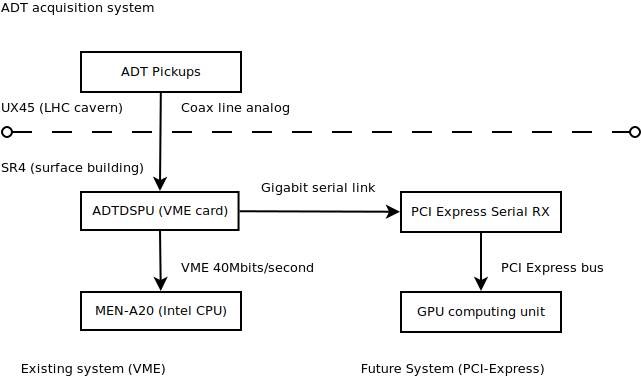
\includegraphics[scale=0.3]{acquisition.pdf}
	\end{figure}

   Per bunch position measurement has to be available to the system for each beam and each plane. This should be provided by the \gls{ADTDSPU} card and has to be transfered through a serial link to the CPU/GPU crate for computation.

   We need a card in the CPU/GPU crate to de-serialize the data and transfer them to the GPU memory. It may be possible to copy from the acquisition card directly to the GPU memory.

   And finally we of course require fast enough GPU to process the data. The number and the type of cards should be carefully looked at. The possibility for expansion should be kept in mind as the possibility to implement other algorithms.
   
   \subsection{Timings}

   According to the \gls{BI} group we have to provide the tune measurement at a rate of between 5 Hz and 10 Hz delay. This mean that the transfer and the computation has to be made in less than 200 ms.

   At a higher frequency because of the acquisition frequency (11 kHz) the precision may be insufficient (Nyquist$-$Shannon sampling theorem).
% Graphic Processing Unit
%
%	Take from the PA

\glsresetall
\chapter{Graphics Processing Unit}

A \gls{GPU} is a specialized chip for outputting an image on a display. They are used in embedded systems, mobile phones, personal computers, workstations, and game consoles. \Glspl{GPU} are presently able to compute 3D images using a custom programmable rendering pipeline. This capacity can be diverted to be used for general purpose computing.

\section{Introduction}

General purpose programming on \glspl{GPU} is a new field with a growing community of practitioners. Until recently only proprietary interfaces existed to harness the power of these chips. With the arrival of the \gls{OpenCL} a new open interface has appeared, and with it a hope for a unified, simple and portable framework for general purpose computing on heterogeneous hardware.

\section{OpenCL}

The \gls{OpenCL} is the open standard for \gls{GPGPU} programming. It is maintained by the Khronos group, and was initially proposed by Apple. Many companies of the industry are members of the \gls{OpenCL} Working group: Altera, AMD, Apple, ARM, Broadcom, Codeplay, DMP, EA, Ericsson, Fixstars, Freescale, Hi corp, IBM, Intel, Imagination Technologies, Kestrel Institute, Kishonti, Los Alamos National Laboratory, Motorola, Movidius, Multicoreware, Nokia, NVIDIA, OpenEye, Presagis, Qualcomm, Rightware, Samsung, ST, Symbio, Texas Instruments, The University of West Australia, Vivante and Xilinx~\cite{opencl}.
\begin{quotation}
``OpenCL\texttrademark is the first open, royalty-free standard for cross-platform, parallel programming of modern processors found in personal computers, servers and hand-held / embedded devices. \gls{OpenCL} greatly improves speed and responsiveness for a wide spectrum of applications in numerous market categories from gaming and entertainment to scientific and medical software.''~\cite{opencl}
\end{quotation}
\begin{quotation}
``The Khronos Group is a not for profit industry consortium creating open standards for the authoring and acceleration of parallel computing, graphics, dynamic media, computer vision and sensor processing on a wide variety of platforms and devices. All Khronos members are able to contribute to the development of Khronos \gls{API} specifications, are empowered to vote at various stages before public deployment, and are able to accelerate the delivery of their cutting-edge 3D platforms and applications through early access to specification drafts and conformance tests.''~\cite{khronos}
\end{quotation}

\subsection{Architecture}

\gls{OpenCL} is not really a language but an \gls{API} and a kernel language derived from C99 that is compiled for, and executed on the device itself. It defines an abstract hardware architecture onto which the real hardware is mapped. Every piece of hardware (\gls{CPU}, \gls{GPU}, others) is called a device. This device is divided into work groups, each of which is further subdivided into work items.

\begin{figure}[H]
\caption{OpenCL Device Model}
\floatfoot{Source : OpenCL in Action~\cite{OpenCLInAction}}
\centering
\includegraphics[scale=0.5]{OpenCL_Device_Model.pdf}
\end{figure}

\subsection{OpenCL API}

The \gls{OpenCL} \gls{API} is composed of two parts: The host code that runs on the CPU which runs kernel handling event synchronization and manages the memory buffer, and the device code, which is a kernel language based on the C99 specification.

\begin{figure}[H]
\caption{Kernel Distribution among OpenCL-compliant devices}
\floatfoot{Source : OpenCL in Action~\cite{OpenCLInAction}}
\centering
\includegraphics[scale=0.5]{OpenCL_Objects.pdf}
\end{figure}

The host \gls{API} is written in C but there is a C++ interface provided by Khronos, which is the interface used in this work. Several other wrappers for other languages are available, such as Java, C\#, Python, and even javascript with WebCL (also specified by the Khronos group). 

The device code also called \gls{OpenCL} ``kernel code'' is based on is C99, adding some extensions like vectorization, image access, and linear algebra functions.

The workload itself is specified in terms of context, program and command queues. The context contains the parameters of the current problem and manages the devices available for computation, as well as the programs and the command queues. The program consists of the set of kernels which are constructed from \gls{OpenCL} code. The context is responsible for dispatching these kernels into command queues. Each command queue is a set of commands that can be executed in any order, or simultaneously. A command queue is limited to a single device~\cite{OpenCLInAction,OpenCLProgrammingGuide}.

Events fired by devices are also available for triggering specific actions in case a finer synchronization mechanism is needed. Once the device has finished, the host receives and processes the output data via the buffer \gls{API}.

\section{Other GPGPU languages}

For the purpose of completeness we present also the other general purpose computing languages used on \glspl{GPU}. Shader languages, the 3D pipeline programming languages used for computer graphic, will also be briefly mentioned. hey are not a real general purpose computing language but are still used for general purpose computing.

\subsection{CUDA}

\Gls{CUDA} is the most widely used interface for general purpose \gls{GPU} programming. It was developed by NVIDIA, has been used for many years and is still very much in use. It only works on NVIDIA \glspl{GPU}, and will not run on other \glspl{GPU} or \glspl{CPU}. Since it is a proprietary language, NVIDIA is in total control of the API and its development kit.

The abstraction level in \gls{CUDA} is less strong than in \gls{OpenCL}, that is, the language is closer to the architecture. This means it could potentially offer more optimization possibilities to the programmer. We will see that this is not a key element as the compiler is able to reach this level of optimization without having to compromise code readability.

\Gls{CUDA} has its kernel and \gls{GPU} code directly embedded inside the C/C++ code. In \gls{OpenCL} the code is separated from the C/C++ host code. This can lead to incompatibilities with C++ as valid C++ code will be flagged as invalid by the \gls{CUDA} compiler. This problem does not exist for \gls{OpenCL} as the compiler is a separate entity and the code is fed to it via the \gls{API}. 

\Gls{CUDA} offers a full suite of libraries and tools that are presently not available in \gls{OpenCL}. Among these are performance tuning tools and libraries for matrices and \glspl{FFT}. Recently many implementations of common algorithms have started to appear for \gls{OpenCL}, and unlike with \gls{CUDA}, these are directly available to any computing device.

\subsection{DirectCompute}

This is the Microsoft interface, strongly tied to the Windows platform. DirectCompute is part of the DirectX API, the game development tools for Windows. It works with DirectX 10 and 11 under Windows Vista and Windows 7. 

DirectCompute shares a lot of concepts with both \gls{CUDA} and \gls{OpenCL}, and is presently working with both AMD and NVIDIA graphic cards.

\subsection{Shader Languages}

Shading are the steps that the graphic card has to take before rendering to the screen. There are two steps: the vertex shader, also called vertex code; and the pixel shader, also called fragment code. The vertex shader is transforms vertex data from 3D space to 2D screen coordinates by manipulating the data as points in space (vectors). The pixel shader is doing the final rendering of pixels on the screen calculating the color of a pixel according to the light, the normal and textures. 

There are many different shader languages. The main ones are: Cg, the NVIDIA ``neutral'' shading language, one of the first languages widely used on \glspl{GPGPU}; the \gls{HLSL}, the Microsoft version tightly coupled with DirectX, and therefore easier to use on a Microsoft platform (XNA); the \gls{GLSL}, an \gls{OpenGL} version, that is supported widely but not implemented completely on all platforms. 

Before the general purpose graphic processing languages appeared shader languages were the only way to access the power of the graphic card, and they are still much in use today. As it was developed over many years, this is a very stable technology and there are many examples and libraries using theses languages.

Shader languages are oriented towards graphics programming and are therefore not well-adapted to some of the algorithms we may want to implement. They are made to handle vectors of four components, such as position, color, texture, and normal vectors.

\section{Environment selected}

The system is going to run on dedicated \gls{CERN} computers that operate under \gls{SLC}. A language running on Linux is thus a must. The ability to test the whole system on a \gls{CPU} and to compare the processing speed is also a key factor. The system should be able to be expanded and not be tied to any hardware provider. \Gls{OpenCL} is then the only choice.


% Results
%
%	some important things to know
% 	experimental parts in the chapter results
%	numerical results or so-called data
%	order of presentation
% 	cross references

\chapter{Results}

\section{FFT}

\begin{figure}
\caption{Spectrogram of the beam position taken on the 16 October 2012}
\centering
\includegraphics[scale=0.2]{spectrogram.pdf}
\end{figure}

\section{SVD}

\section{FFT uing GPU}

   \subsection{Performances}

\begin{figure}
\caption{Time flow with different implementations and with 3000 bunches of 
2048 points each.}
\centering
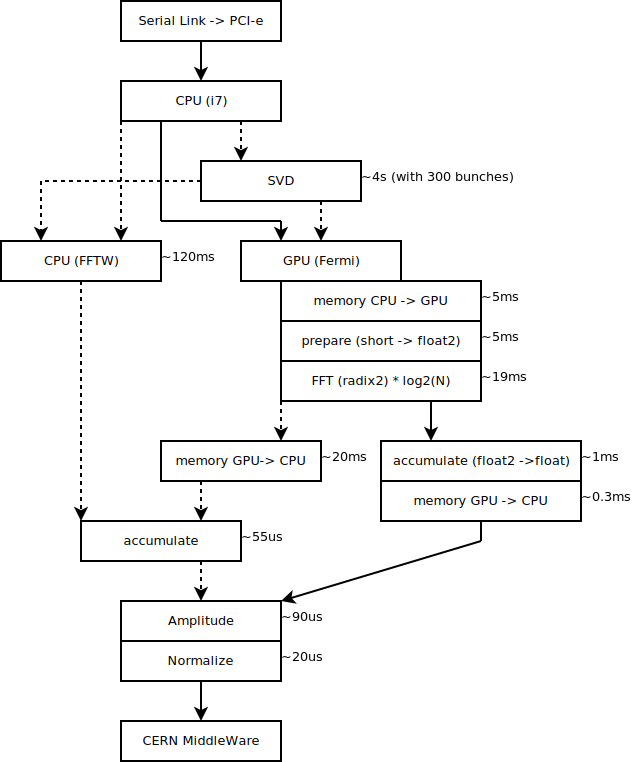
\includegraphics[scale=0.4]{PC-flow.pdf}
\end{figure}

   \subsection{Pipelining}

   Pipelining was tested and used in the process and it was possible to
   win around 15\% in performances around it.

   \subsection{Memory}


% Discussion

\chapter{Discussion}

With All these result the tune can be assumed to be visible and it is then possible to assess the feasibility of the tune measurement using \gls{GPU}. There is still some question around hardware update but the work left to be done can be fairly well estimated.

\section{Observation}

During the three \gls{MD} we acquired around TODO with both beam and both planes. This data was acquired in XML files and stored on the \gls{CERN} infrastructure. XML was chosen as it is easily accessible by both custom and commercial data analysis software.

Matlab was used as the first tool to check the data and try different algorithm but in the end the software was ready fast enough and flexible enough. Matlab ended to be only used for check and test purpose and all the analysis and discussion is based on the result obtain with the data analysis software described in section~\ref{sec:data_analysis_software}.

	\subsection{Without damper}

	When the \gls{ADT} is off line there is a clear mark on the tune as shown in Figure~\ref{fig:adt_off}. There is still discussion on is it the tune or just a ripple of the tune but as when the tune is moved the mark is also moving it is safe to assume this is really the tune. Some test could still be made, crosschecking with the \gls{BBQ}, changing the tune and looking in real time.

	\begin{figure}[H]
	\caption{Spectrogram with ADT off on the 16 October 2012 on vertical beam 1 before the ramp, 6 bunches 10 accumulations}
	\label{fig:adt_off}
	\centering
	\includegraphics[scale=0.3]{md-121016-vb1-m1-6bunches-10acc-1337-1349-ADT-off.pdf}
	\end{figure}

	These observations are consistent with the gated-\gls{BBQ} result of 2012 \cite{Valuch12} and show that we can acquire the tune with the \gls{ADT} and get a clear bunch-by-bunch view of the tune even for only one bunch as shown in Figure~\ref{fig:bunch_0_adt_off}.

	\begin{figure}[H]
	\caption{Spectrogram with ADT off on the 16 October 2012 on horizontal beam 1 before the ramp, 1 bunch (0) 8 accumulations}
	\label{fig:bunch_0_adt_off}
	\centering
	\includegraphics[scale=0.3]{md-121016-hb1-m1-bunch000001-8acc-1337-1349.pdf}
	\end{figure}

	\subsection{With damper}

	When the \gls{ADT} is working the oscillations of the beam are damped by it, as a result the tune is less visible. But we should be able to see the effect of the tune on the damper if the damper is well adjusted to the beam. This mean that we should see a clear gap in the frequency around the tune frequency (or at the frequency the damper is less working, frequency that should correspond to the tune).

	This correspond to the spectrogram we see during operation as shown in Figure~\ref{fig:ramp}. We also see in this figure the ramp that lead to collision, before putting the beam in collision we do a squeeze (operation during witch we compress the beam size in the interaction points, where the experiments are). The squeeze is changing the tune and we can see it on the spectrogram around 14h03 on the figure \ref{fig:ramp}.

	\begin{figure}[H]
	\caption{Spectrogram with damper working on the 16 October 2012 on vertical beam 1 during the ramp, 6 bunches 10 accumulations}
	\centering
	\label{fig:ramp}
	\includegraphics[scale=0.3]{md-121016-vb1-m1-6bunches-10acc-1347-1405-ramp.pdf}
	\end{figure}

	This could give us a good acquisition of the tune during operation even when \gls{ADT} is on. This acquisition could be made bunch-by-bunch so we could correct position of bunches that are not well on tune. The question that is still up is how much is it sensible to the way the \gls{ADT} is set up. This has still to be tested in the machine by moving the tune while the \gls{ADT} is in operation and see if the acquisitions follows the tune.

\section{Data flow}

As the hardware is not present yet, the time and bandwidth of the whole system has to be estimated to see if it is doable in the constraint we have and that were exposed in the introduction. Estimation of the bandwidth and data flow is shown in Figure~\ref{fig:data_flow}.

\begin{figure}[H]
\caption{Acquisition data flow}
\label{fig:data_flow}
\centering
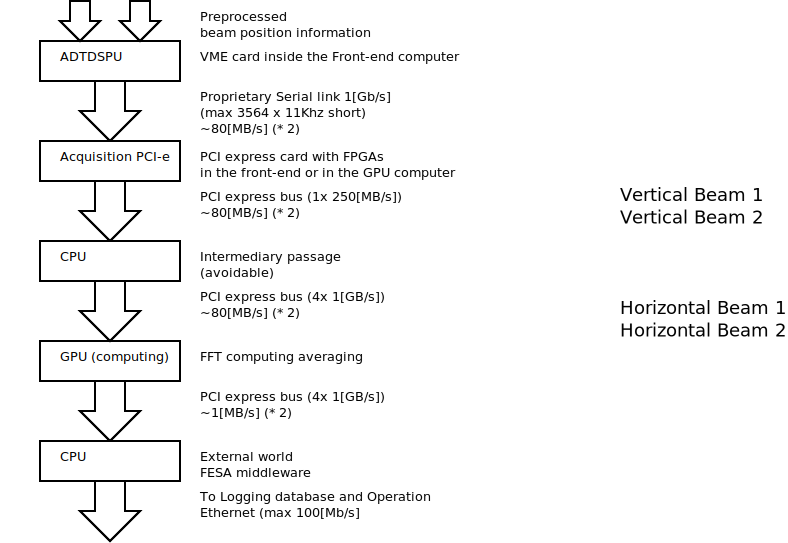
\includegraphics[scale=0.3]{dataflow.pdf}
\end{figure}

The data has to move from the acquisition card to the GPU by a series of steps, first from the card to the PCI crate (the one who contain the actual \glspl{GPU}). The problem being that the acquisition card is a \gls{VME} card and the VME bus is too slow to allow the full data to be streamed to the CPU. This will use the Giga-bit serial link already present on the VME card. A receiver card will then receive the data in the PCI crate and send it either directly to the \gls{GPU} memory or to the \gls{CPU} and then to the \gls{GPU} memory. Then the \gls{GPU} will make the computations necessary for the tune measurement and will copy back to the \gls{CPU} that will use the normal Ethernet connection to stream it back to operation.

\section{Hardware}

The present hardware is not allowing to acquire all the \glspl{bunch} of the machine and is in fact limited by constraints of the \gls{VME}. We have to upgrade various part of the hardware and to add the new computing device in order to be able to make on-line computation of the tune.

	\subsection{ADT Acquisition boards}

	The ADTDSPU card has to be upgraded?! (TODO check with Daniel)

	\subsection{Serial link interface}

	Serial link receiver has to be chosen and put into place in the new computing device to be able to receive the data and pass them to the \gls{GPU}. (TODO check with Daniel on what spec, what speed...).

	Talk about market survey with Daniel. development of the FPGA firmware, show figure.

	Talk about the in-house solution with the CO card, show figure.

	\subsection{GPUs}

	We need a computing device with at least 2 PCIe slots, one for the serial link receiver and one for the \gls{GPU} card. It should be some standardized crate with a powerful \gls{CPU} and possible expansion. Place has to be checked in SR4 to check if there is enough space for full crate or we have to take lighter crates.

\section{Software}

Some software upgrade and redeployment is still necessary before the operational version is fully commissioned.

	\subsection{Drivers}

	The drivers for the \gls{ADT} acquisition card will need some update, changing the memory map and adjusting the drivers for the control registers. This should be quite straightforward.

	A driver for the Serial link receiver card will be needed, either, if we use one that is made inside \gls{CERN} we can have it made by the control group (CO). Or in case we buy an off the shelf solution we will have to make the driver ourself using the driver framework and the tools we have.

	\subsection{OpenCL}

	The present \gls{OpenCL} code is able to compute the \gls{FFT} but we could try other algorithms in the future including hardware accelerated \gls{SVD}. This would ask some new \gls{OpenCL} development.

	\subsection{Front-end}

	

\section{Estimated Cost}

	\subsection{First prototype}

	\subsection{At LHC restart}
% conclusion

\chapter{Conclusion}

\glsreset{GPU}
\glsreset{FFT}
\glsreset{LHC}

The betatron \gls{tune} is a critical parameter of a particle collider machine. In the \gls{LHC} the \gls{tune} acquisition is computed by doing \glspl{FFT} on an averaged value over all the bunches. In order to have a decent on-line \gls{FFT} computation of all individual bunches a faster method is needed. 

\Gls{GPU} used in graphic card are faster than normal \gls{CPU} for parallelized computations. Using a \gls{GPU} we can accelerate \gls{FFT} computation by a factor of 10 especially if we have multiples \glspl{FFT} to be computed at the same time. This could, acording to the timing asked by the operation, allow for a new on-line bunch-by-bunch acquisition of the \gls{tune}.

New hardware will have to be deployed in the \gls{ADT} Faraday cage. This will in turn need new software to drive it. But is should be accessible as most of it is already present in the \gls{ADT} setup.

On-line computation of \glspl{FFT} for all the individual bunch is shown to be possible this will allow a better bunch-by-bunch surveillance of the beam and better statistic on what is causing transversal instabilities. This could allow to have a better tune acquisition and allow for a better beam time life in the \gls{LHC}.
\include{annex}

\printglossaries
\bibliographystyle{plain}
\bibliography{bibliography}

\end{document}

